\documentclass[11pt]{article}
\usepackage[margin=1in]{geometry}
\usepackage{amsmath,amssymb}
\usepackage{graphicx}
\usepackage{booktabs}
\usepackage{tabularx}
\usepackage{enumitem}
\usepackage{hyperref}

\setlength{\emergencystretch}{2em}

\title{A Source-Frozen Decision Protocol for Dark-Sector Necessity in Tau Core Galaxy Rotation}
\author{Jozsef Olcsak\\{\small ORCID: \href{https://orcid.org/0009-0003-7311-6522}{0009-0003-7311-6522}}}
\date{Last revised: 14 November 2026}

\begin{document}
\maketitle

\begin{abstract}
This paper defines a source-frozen, galaxy-scope decision protocol for testing dark-sector necessity across three declared model families: a no-dark Tau morphology/readout endpoint ($M_0$), a Tau base-substrate response endpoint ($M_1$), and a standard dark-sector benchmark ($M_2$). Rather than claiming a global proof or rejection of dark matter, the protocol renders the narrower galaxy-rotation question decidable under pre-registered sample roles, shared held-out scoring rules, parsimony accounting, and leakage controls that forbid residual feedback before activation. In its canonical \texttt{v82} state, the repository completes source-side provenance verification, raw SPARC import ($450$ radial rows across $18$ frozen galaxies), and $72$-component prescore leakage certification, emits the non-scored $M_0$ baryonic anchor table $v_{\mathrm{body}}(R):=v_{\mathrm{anchor}}(R)$, and freezes protocol-local parameter and per-galaxy privilege counts at zero across $M_0$, $M_1$, and $M_2$, leaving the shared-input count-discount policy (\path{shared_input_count_discount_policy_v10.csv}), unconstructed $M_1/M_2$ prediction tables, control runners, and numerical decision cutoffs as explicit pre-scoring gates. No $\mathrm{Response}_{\tau}$ law, $S_{\tau}^{\mathrm{resp}}$ functional, or endpoint verdict is claimed here; upstream zero-parameter $171$-galaxy SPARC and high-redshift OCSR benchmarks are documented separately without activating Paper~11 endpoint scoring.
\end{abstract}

\section{Scope}

The decision question is:
\[
\text{Does the declared galaxy-rotation endpoint class require a dark-sector
response layer?}
\]
The answer is restricted to the tested endpoint class. It is not a global
claim about dark matter, dark energy, lensing, CMB, BAO, growth, or cosmology.
The protocol is intended to sit downstream of the Tau Core theory architecture
and the Paper 9--10 freeze/readout scaffolds
\cite{tauCoreTheoryHub2026,tauCorePaper9,tauCorePaper10}.

In the current Tau Core terminology, the source-side object behind any
no-dark morphology/readout endpoint is the \emph{morphological body}
\(M_\tau\).  The galaxy labels and kernels used by a decision protocol are
projected/source-frozen handles on that body, not a claim that visible
four-dimensional morphology exhausts the source.

\section{Theory-Side Scoring Anchor}

The Tau Core theory hub now supplies a restricted local scoring anchor that is
relevant to this protocol but does not itself score galaxies. The anchor is the
finite-local \(U_{\mathrm{read}}\) closure-defect partial-order diagnostic
\cite{tauCoreTheoryHub2026}:
\[
\begin{aligned}
\Theta_{\mathrm{vec}}(c)=(&
\mathrm{rank}_{\mathrm{status}}(\mathrm{ClosureStatus}(c)),\\
&\mathrm{rank}_{\mathrm{obstruction}}(\mathrm{ClosureObstruction}(c)),\\
&\mathrm{rank}_{\mathrm{mismatch}}(\mathrm{ClosureMismatch}(c))).
\end{aligned}
\]
and local relation
\[
c_i \leq_{\mathrm{read}} c_j
\quad\Longleftrightarrow\quad
\Theta_{\mathrm{vec}}(c_i)\geq_D \Theta_{\mathrm{vec}}(c_j).
\]
The hub records this object as a restricted formal local order-readout
admissibility pass under stated assumptions. The pass is conditioned on
family non-circularity, observer-interface admissibility, null/gauge
preservation, conservative \(\mathrm{CG}_{\mathrm{read}}\) stability, and a
reported partial-order incomparability envelope.

For Paper 11, this result is a theory-side scoring primitive: it shows that a
local Tau Core scoring/readout object can be made source-frozen,
non-circular, observer-interface guarded, null/gauge compatible,
coarse-graining conservative, and explicit about incomparability. It does not activate endpoint scoring, construct the galaxy endpoint score, fill family
prediction tables, decide between \(M_0,M_1,M_2\), prove physical time, or
establish a physical readout.

The latest Tau Core theory-hub work also supplies a separate local
\(K_{\mathrm{time}}\) audit pattern from the CERN/SPS chain: local nonphysical
transport can feed a finite carrier family, and the declared local labels can
be transported conditionally into standardized rank domains without erasing
missing-proof, proxy-residual, or bridge-boundary information. For this paper
that result is only a methodological guardrail for scoring design. It supports
the separation of carrier recognition, rank-domain transport, and later
\(\Theta_{\mathrm{time}}\)-like vector evaluation. It does not prove
\(\Theta_{\mathrm{time}}\) totality, a preorder for galaxy data, a physical
readout, or physical time.

\section{Paper 10 Shape/Readout Consequence}

The most relevant upstream Paper 10 update for Paper 11 is not a positive
cosmological validation claim. It is a design constraint: level/amplitude
support and shape/readout support must remain separate. In the DESI
time/readout route, the constant-level DESI--chronometer replay is
ordering-fragile under frozen controls, so it cannot be used as a scoring
shortcut. The shape/readout route is more informative: Paper 10 records a
source-strengthened but narrow and row-sensitive DESI shape-core support
synthesis, with row-level caveats reduced but no endpoint validation
\cite{tauCorePaper10}.

For Paper 11 this means that the family comparison must not reward a model
merely for absorbing a residual level. The \(M_0\) no-dark family must forbid
hidden dark-sector compensation coefficients, the \(M_1\) Tau base-substrate
response family must declare response channels before endpoint scoring, and
the \(M_2\) standard dark-sector benchmark must be compared with controls that
distinguish amplitude improvement from shape/control resistance. This update
does not activate scoring and does not favor \(M_0\), \(M_1\), or \(M_2\).

\section{Blocked Full-4D Readout Subfamily}

The observer-specific Tau 4D descent adds a transport-completion tag to the
existing Tau families; it is not a fourth family chosen after endpoint access.
For \(a\in\{0,1\}\), let \(M_a^{4D}\subset M_a\) denote the subfamily for
which one source-derived radial relative coframe \(D_O(R)\) induces
\begin{equation}
 g_O^\tau=(e_O^{\rm GR})^*D_O^*\eta D_Oe_O^{\rm GR}
 \longleftrightarrow
 \bigl(N_O,\beta_O^i,q_{ij}^{(O)}\bigr)
 \label{eq:paper11-full-4d-descent}
\end{equation}
and supplies the associated null/photon transfer.  On an equatorial circular
path the local speed must obey
\begin{equation}
 v_{O,{\rm local}}^2(R)
 =\frac{q_{\phi\phi}^{(O)}(R)}{N_O^2(R)}
 \left[\Omega(R)+\beta_O^\phi(R)\right]^2,
 \label{eq:paper11-full-4d-local-speed}
\end{equation}
while the scored spectral estimator must be declared separately from the same
metric and photon path.

This subfamily is blocked.  It may be activated only when \(D_O(R)\), its
support, coefficients, null/gauge policy, parameter budget, and spectral
transfer are frozen without target rotation residuals; the exact \(D_O=I\)
branch is included; and time-only, spatial-only, shift-only, full-coframe and
standard-systematics controls are executable.  At least one non-rotation
readout consequence from the same \(D_O\) is required to prevent a relabelled
rotation-only fit.  The current paper supplies none of these numerical fields,
so this section changes no activation row, family score, or decision status.

Even after activation, the positive mixed-Hessian Schur term is not itself a
dark-sector prediction.  With a standard same-support comparator the exact
source excess is
\[
 E_K=(K_{HH}-K_{\rm std})-CK_{VV}^{-1}C^\dagger.
\]
The graph-normal \(C\neq0\), \(E_K=0\) control is mandatory.  A future
family comparison may score only the frozen multi-terminal image of a nonzero
\(E_K\), with exact duplicate directions removed and the full joint covariance
retained.  This compiler sharpens the blocked contract but supplies no current
prediction or score.

For the shift-only control, common-packet co-registration conditionally fixes
the oriented row
\[
 q_\tau
 =-\omega_{uv}P_\beta\mathcal L_O^{-1}B_{OS}^{*}W_\rho
   (D_BCx+D_Aa),
\]
and standard photon-rapidity occupation would imply
\[
 h_\tau
 =c\,\frac{(1-\beta_{\rm dyn}^{2})\tanh q_\tau}{1+\beta_{\rm dyn}\tanh q_\tau}.
\]
This removes an arbitrary post-source velocity gain from that declared
ablation, but does not activate \(M_0^{4D}\) or \(M_1^{4D}\).  A rotation
terminal alone cannot identify whether a common row arose from body morphology
or irreducible observer--source access.  Paper~11 must therefore freeze a
stable \(Q_{OS}\) and a complete joint terminal law whose resolved partition
separates those contributions; duplicated or factorized readouts do not count
as new information.  Nonzero joint incidence, orientation, calibration,
standard-orthogonal survival and Nature occupation all remain open.

\section{External Readout-Time Motivation}

Recent quantum-optical weak-measurement work gives an external motivation for
treating time-like quantities as protocol/readout dependent observables rather
than always as direct classical residence times. Angulo et al. report negative
weak values for the time atoms spend in the excited state when a photon is
transmitted through an atom cloud, using a cross-Kerr probe and comparing the
inferred atomic-excitation time with group delay
\cite{anguloNegativeWeakTime2026}. This is not time travel, not
faster-than-light signalling, and not evidence for Tau Core. Its role here is
methodological only: it supports the caution that a time-like measured
quantity can depend on the source state, observer/readout interface, scale,
post-selection, and null model. Paper 11 therefore treats galaxy endpoint
readouts as declared protocol objects, not as automatically physical
readouts.

\section{Model Families}

The protocol compares three families:
\[
M_0 = \text{no-dark Tau morphology/readout},
\]
\[
M_1 = \text{Tau base-substrate response},
\]
\[
M_2 = \text{standard dark-sector benchmark}.
\]
The \(M_1\) family uses ``Tau dark sector'' only as an internal name for a Tau
base-substrate response layer. It is not identified with a standard particle
dark-matter or dark-energy fluid.

\section{Freeze Discipline}

All source, policy, and family choices must be frozen before endpoint scoring.
In particular,
\[
\mathrm{Freeze}(\text{policy bundle}) < \mathrm{Score}(\text{endpoint}).
\]
Endpoint residuals, best-fit curves, held-out scores, and pass/fail labels are
forbidden inputs for source definition, state-kind selection, admissibility,
term selection, stable selection, and channel handoff.

\section{Decision Outcomes}

If \(M_0\) wins held-out tests with controls, the allowed interpretation is
that a no-dark Tau endpoint is sufficient for the declared galaxy-rotation
endpoint class. This is not a global rejection of dark matter.

If \(M_1\) wins, the allowed interpretation is that a Tau base-substrate
response layer is favored for the declared endpoint class. This is not a proof
of a physical Tau dark-sector field.

If \(M_2\) wins, the allowed interpretation is that the standard dark-sector
benchmark remains stronger for the declared endpoint class. This is not a
global falsification of Tau Core.

\section{Current Status}

The present repository supplies a decision-protocol scaffold, a frozen-reference
policy-bundle instance \(PB11\_v01\), a first galaxy endpoint decision
manifest, and structured pre-registration, provenance, leakage-certification,
formula-contract, and parameter-count ledgers culminating in canonical state
\texttt{v82}. While row-level source inputs and the non-scored \(M_0\) baryonic
anchor table are populated, endpoint scoring remains blocked by unactivated
\(M_1/M_2\) prediction tables, shared-input count-discount policy, executable
control runners, and numerical decision thresholds. The following remain absent:
\[
\begin{aligned}
&\mathrm{Response}_{\tau}, \quad
S_{\tau}^{\mathrm{resp}},\\
&\mathrm{Select}_{\mathrm{stab}}, \quad
\mathrm{ChannelHandoff}_{\tau},
\end{aligned}
\]
as constructed mathematical objects. No endpoint result is reported.

\section{Decision Manifests: Canonical \texttt{v82} Architecture}
\label{sec:decision-manifests}

Across protocol revisions \texttt{v01} through \texttt{v82}, the repository
decomposes the pre-scoring freeze into six auditable dependency tracks so that
source import, leakage review, formula-body assembly, and parameter-budget
accounting are each verified independently before any endpoint comparison can
execute. Table~\ref{tab:v82-architecture} summarizes the canonical \texttt{v82}
state of each track.

\begin{table}[ht!]
\centering
\caption{Canonical \texttt{v82} pre-scoring manifest architecture across the six Paper~11 dependency tracks.}
\label{tab:v82-architecture}
\footnotesize
\renewcommand{\arraystretch}{1.18}
\begin{tabularx}{\textwidth}{@{}>{\raggedright\arraybackslash}p{2.5cm} >{\raggedright\arraybackslash}p{2.3cm} >{\raggedright\arraybackslash}X >{\raggedright\arraybackslash}p{2.7cm}@{}}
\toprule
\textbf{Track} & \textbf{Ledger span} & \textbf{Scope and canonical artifacts} & \textbf{\texttt{v82} status} \\
\midrule
1.\ Policy \& roles & \texttt{PB11\_v01}, \texttt{v01--v07} & Three-family roles ($M_0,M_1,M_2$), five sample roles, six score components, six control contracts, and preflight blocker audit. & Policy frozen; scoring blocked \\
2.\ Provenance \& import & \texttt{v08--v36}, \texttt{v44--v57} & SHA-256 verified SPARC provenance (\texttt{source\_\allowbreak{}import\_\allowbreak{}provenance\_\allowbreak{}evidence\_\allowbreak{}v21.csv}) and authorized raw/real import (\texttt{source\_\allowbreak{}import\_\allowbreak{}real\_\allowbreak{}values\_\allowbreak{}v12.csv}: $18$ galaxies, $450$ rows). & $18/18$ galaxies imported \\
3.\ Leakage \& activation & \texttt{v37--v43}, \texttt{v58--v79} & Four-component prescore leakage review across all $18$ galaxies ($72$ rows in \texttt{leakage\_\allowbreak{}audit\_\allowbreak{}evidence\_\allowbreak{}v10.csv}) and row-level gate activation (\texttt{v79}). & $72/72$ certified; $18$ rows active \\
4.\ Family formula tables & \texttt{v06--v14}, \texttt{v80--v81} & Non-scored $M_0$ baryonic anchor $v_{\mathrm{body}}(R):=v_{\mathrm{anchor}}(R)$ ($450$ rows emitted into \texttt{family\_\allowbreak{}prediction\_\allowbreak{}tables\_\allowbreak{}v08.csv}); $M_1$ response/admissibility and $M_2$ profile/nuisance slots held as no-values contracts. & $M_0$ emitted; $M_1,M_2$ unfilled \\
5.\ Parameter \& privilege budgets & \texttt{v06--v15} ($M_0,M_1,M_2$) & Global slot inventories, adjustability resolutions, and per-galaxy privilege audits freezing protocol-local $k_{\mathrm{global}}=0$ and $0/18$ row privileges across $M_0,M_1,M_2$. & Next gate: \texttt{shared\_\allowbreak{}input\_\allowbreak{}v10} \\
6.\ Upstream scoring guards & \texttt{v81--v82} & Local $U_{\mathrm{read}}$ partial-order primitive, $K_{\mathrm{time}}$ rank-domain discipline, and Paper~10 level-vs.-shape control guardrails. & Guardrails active; no scoring \\
\bottomrule
\end{tabularx}
\end{table}

\paragraph{Tracks 1--3: Pre-registration, SPARC provenance, and 72-row leakage certification.}
The foundational policy bundle \texttt{PB11\_v01} and layers \texttt{v01--v07}
freeze the five sample roles (train, held-out, control, challenge, and
transfer-candidate), six scoring components (full curve, inner zone, outer
zone, parsimony, held-out median, and control veto), and six control gates
(shuffled-label, wrong-family, null-source, leakage, radial-zone, and
family-budget parity) without selecting numerical cutoffs. Following template
scaffolding (\texttt{v08--v25}), independent SHA-256 recomputation and
two-stage human-review intake (\texttt{v44--v55}; preserving \texttt{v26--v34}
as superseded historical work orders) populate all $18$ candidate SPARC
provenance records in \path{data/input/source_import_provenance_evidence_v21.csv},
enabling the authorized raw MassModels adapter (\texttt{v56--v57}, \texttt{v17})
to write $450$ radial velocity rows into
\path{data/input/source_import_real_values_v12.csv}. Layers \texttt{v58--v78}
then expand the \texttt{v10} leakage contract into $72$ prescore verification
items ($4$ components $\times$ $18$ galaxies: source route, observed input,
morphology-label policy, and benchmark-policy isolation), auditing and writing
all $72$ certified rows to \path{data/input/leakage_audit_evidence_v10.csv} so
that the \texttt{v79} row-activation gate marks all $18$ galaxy rows ready for
downstream prerequisites while keeping endpoint scoring disabled.

\paragraph{Track 4: Family formula contracts and $M_0$ baryonic anchor emission.}
With source-side rows certified, the \texttt{v41} and \texttt{v80--v81}
dependency traces move the active frontier to
\texttt{SCD24\_FAMILY\_FORMULA\_TABLES} (\path{family_prediction_tables_v08.csv}).
Across the $M_0$ derivation chain (\texttt{v06--v14}), symbol-binding,
dimensional-anchor, unit-normalization, and component-weight freezes fix the
purely baryonic source-side velocity anchor
\begin{equation}
v_{\mathrm{anchor}}^2 =
\frac{s_{\mathrm{gas}}w_{\mathrm{gas}}v_{\mathrm{gas}}^2
+s_{\mathrm{disk}}w_{\mathrm{disk}}v_{\mathrm{disk}}^2
+s_{\mathrm{bulge}}w_{\mathrm{bulge}}v_{\mathrm{bulge}}^2}
{n_{\mathrm{anchor}}}\,,
\qquad
v_{\mathrm{body}}(R) := v_{\mathrm{anchor}}(R)\,,
\label{eq:paper11-m0-baryonic-anchor}
\end{equation}
and \path{m0_no_dark_family_prediction_row_emission_v08} emits the resulting
$450$ non-scored $M_0$ rows alongside the frozen morphology-label rule contract
(\path{m0_label_rule_table_v06}). By contrast, the $M_1$ response-slot and
admissibility contracts (\path{m1_tau_response_formula_table_v06},
\path{m1_admissibility_table_v06}), the $M_2$ halo-profile and nuisance-policy
contracts (\path{m2_benchmark_profile_table_v06},
\path{m2_nuisance_policy_table_v06}), and the shared scoring-input contract
(\path{shared_scoring_input_table_v06}) remain closed as pre-scoring
no-values/no-predictions scaffolds.

\paragraph{Tracks 5--6: Protocol-local parameter freezes and \texttt{v81--v82} upstream guards.}
To prevent hidden flexibility in future parsimony comparisons, the
count-readiness decomposition (\path{numeric_count_readiness_closure_v09.csv})
audits global slot inventories (\texttt{v10}), countability classifications
(\texttt{v11}), value ledgers (\texttt{v12}), conditional-slot resolutions
(\texttt{v13}), and final-count freezes (\texttt{v14--v15}) together with
$18$-galaxy row-privilege audits (\texttt{v10--v11}) across all three model
families ($6$ global slots in $M_0$, $6$ response slots in $M_1$, and $12$
profile/nuisance slots in $M_2$). Under the current no-values scaffold for
$M_1$ and $M_2$ and the fixed baryonic anchor for $M_0$, protocol-local global
counts freeze at $k_{\mathrm{M0,global}}=k_{M1,\mathrm{global}}=k_{\mathrm{M2,global}}=0$
with $0/18$ per-galaxy privileges in every family, advancing the active
count-readiness blocker to \path{shared_input_count_discount_policy_v10.csv}.
Finally, the \texttt{v81} theory-side scoring anchor imports the restricted
local $U_{\mathrm{read}}$ partial-order primitive (It does not activate
endpoint scoring, fill $M_1/M_2$ predictions, or construct
$\mathrm{Response}_{\tau}$), and the \texttt{v82} upstream-impact ledger binds
Paper~10's separation of level/amplitude absorption from shape/control
resistance together with local $K_{\mathrm{time}}$ rank-domain discipline.

\section{Claim Boundary}

This paper does not claim:
\begin{itemize}
\item that dark matter does not exist;
\item that Tau Core replaces the standard dark sector;
\item that a Tau dark-sector physical field is proved;
\item that galaxy rotation, lensing, CMB, BAO, growth, or cosmology are solved;
\item that a \(\mathrm{Response}_{\tau}\) formula or
\(S_{\tau}^{\mathrm{resp}}\) functional has been constructed;
\item that external protocol-dependent time measurements validate Tau Core,
prove physical time, or supply a galaxy-readout formula;
\item that the restricted local \(U_{\mathrm{read}}\) scoring anchor proves
global \(P_{\mathrm{order}}\), physical time, physical readout, or a galaxy
endpoint verdict;
\item that a nonzero galaxy residual, a morphology-matched score, or a
null/time split reconstructs a parent source arrow, a full body connection, or
a varying source-owned access projector;
\item that Paper 10 DESI shape/readout support or Tau Core local
\(K_{\mathrm{time}}\) rank-domain closure proves a dark-sector decision,
physical readout, or endpoint score;
\item that the blocked full-4D subfamily supplies a source-derived nonzero
\(D_O(R)\), activates scoring, or detects non-Einsteinian Tau distortion.
\end{itemize}

\section{Upstream Theory Synchronization and Benchmark Boundary}
\label{sec:upstream-sync}

% BEGIN OBSERVER UPDATE 20260914
\subsection{Observer realization: inherited results and physical boundary}
\label{sec:observer-update-20260914}
The current observer programme distinguishes a conditional mathematical
construction from an occupied physical measuring system. The source order
remains base plus one universal seed, stabilized morphological response,
observer--source restriction, shared descriptor, and resolved terminal
readouts. Neither a detector nor an empirical residual constructs the parent
body backwards. Dynamics below concern downstream subsystems only.

Technical Paper TD-II (Body-to-Readout Derivation) owns the following
results. The existing joint source action fixes static and frequency-dependent
response together. Variation of the BRAC potential couples to the field
square; a linear field coupling is a distinct comparator unless derived by
expansion about an occupied background. Fixed canonical means select a unique
coherent state in a finite positive harmonic packet only if there is no excess
fluctuation energy. This is a free/asymptotic preparation statement, not the
ground state of an interacting detector. For the existing coupled harmonic
pair, the joint ground is pure but either local subsystem is mixed, with its
covariance fixed by the complete joint Hamiltonian.

These are conditional derivations and internal numerical checks. The actual
observer--source context, physical preparation process, kinetic/energy
calibration and stable operational resolution remain unproved. The existing
ORA-T1 selector conditionally chooses stable quantizers when the occupied
context, admissible partition family and positive closure barrier are supplied;
it does not establish those physical premises. A computed ground state is not
a preparation mechanism, and a covariance or optimal abstract measurement is
not an implemented stable quantizer $Q_{OS}$.

\paragraph{Ownership and use.}
The central observer-origin note owns the contact, state and covariance
derivations; Technical Paper TD-II (Body-to-Readout Derivation) carries the consolidated
mathematics. Foundation Papers IV, V and VI retain physical-selection,
clock-descent and quantum-readout ownership, respectively. This paper imports
only the consequences within its scope. No observational dataset, baseline,
frozen coefficient, score or empirical conclusion is revised by this update.
The reproducibility supplement records the source hashes and the exact
conditional/physical distinction.

\paragraph{Consequence for this paper.}
For galactic inference, these observer constructions do not derive a rotation-curve correction or identify a measured residual as a parent effect. Existing endpoint freezes and scores are unchanged.
% END OBSERVER UPDATE 20260914

% BEGIN LAB UPDATE 20260915
\subsection{Finite source-to-readout implementation and its scope}
The current finite laboratory is a reproducible implementation, not a new Nature-selection theorem. The modular family search ranks source-side finite conditioning, not galaxy residuals. The separate galaxy-training mode retains an explicitly supplied spectral-log terminal completion; previously exposed or training galaxies are not fresh validation systems. Neither improving a training curve nor changing graph size establishes morphology ownership, a dark-sector explanation or a Tau-specific residual. Published endpoint rules and scores are unchanged.
\paragraph{Ownership and reproducibility.}
The seed--body companion owns the finite minimum/Hessian example, Technical Paper TD-II (Body-to-Readout Derivation) its ordered access and contact reduction, and the terminal companion its conditional propagation boundary. The physical-source papers retain the source-selection obligation. Code, declared priors, adverse controls and provenance are available at \url{https://github.com/tau-core-research/tau-core-theory/tree/main/experiments/seed_evolution_lab}. Numerical tests are internal evidence only; no published empirical score is changed.
% END LAB UPDATE 20260915

% BEGIN STATE UPDATE 20260918
\subsection{Source identification and recovery}
The current observer audit separates a conditional forward construction from physical source selection. A frozen body, occupied observer incidence, preparation, complete instrument and stable resolution can determine records without selecting those inputs from Nature. Equal effects do not fix postmeasurement states, and symmetry within a chosen interaction family does not exclude other symmetric couplings. For galactic inference, these observer constructions do not derive a rotation-curve correction or identify a measured residual as a parent effect. Existing endpoint freezes and scores are unchanged.

\paragraph{Dependency and claim ownership.}
Foundation VI and Technical Paper TD-II (Body-to-Readout Derivation) own the finite instrument/access proof; Foundation IV and TD-0 retain physical source selection; Foundation V, the temporal synthesis and seed--body companion own the gradient/inertial distinction. This paper inherits only the stated specialization. Canonical assumptions, countermodels and calibration audits are in \url{https://github.com/tau-core-research/tau-core-theory/blob/main/docs/tau_rqm_instrument_to_record_bridge_001.md}. No physical seed, Nature occupation or Tau-exclusive observation is established by this update. Existing empirical endpoint definitions and scores are unchanged.
% END STATE UPDATE 20260918

% BEGIN PAIR READOUT UPDATE 20260927
\paragraph{Imported result (CPR1).}
\href{https://github.com/tau-core-research/tau-core-higgs-module-paper4/blob/main/paper4_full_derivation/full_derivation.pdf#nameddest=cpr1}{Paper 4, \emph{Full Derivation Ledger for the Branch A Higgs Module}}, section ``Conditional source preparation and time-resolved access, Theorem CPR1(b,c)'' v1.0 (2026-09-28), is the sole proof owner.
The imported access-specific result is not a galaxy rotation law or an empirical correction. The frozen galactic construction and every endpoint score remain unchanged; this finite quantum model cannot identify a galactic residual as a parent effect.
Physical preparation, detector/clock calibration and stable $Q_{OS}$ remain assumptions; no Tau-exclusive observation follows.
% END PAIR READOUT UPDATE 20260927

% BEGIN FOUNDATIONS UPDATE 20260929
\subsection{Upstream OCSR-H1 galactic rotation, extended-disk interpolation, and three-pillar closures}
\label{sec:upstream-ocsr-galactic-20260929}

In the upstream theory hub (\texttt{F21--F49} and the 14 November 2026 canonical mathematical unification), analytical closures and empirical benchmark audits have been completed on the $K_4$ branch without modifying the frozen Paper~11 gates:
\begin{enumerate}[leftmargin=1.8em]
\item \textbf{Three-pillar canonical unification (\textbf{Theorems U1--U4}, \textbf{F1--F4}, \texttt{COV-DIR}, \texttt{HOMOG-K4}):}
First, Chung's normalized Laplacian on $K_4$, $\widehat{\Delta}_{K_4}=I_4-D^{-1/2}AD^{-1/2}=\frac{4}{3}P_\perp$, equals the $4\times 4$ Clifford Gram matrix $G_{ij}=\frac{1}{4}\operatorname{Tr}(e_i e_j^\dagger)$ (\textbf{Theorem U1}), making convention \texttt{C2} algebraically identical to \texttt{C1} and fixing $r_{\mathrm{seed}}=1/4$, $\alpha_{\mathrm{OCSR}}=\operatorname{Tr}((I_4-H_b)_+)=5\sqrt{3}/24\approx 0.360843918$ (\texttt{OCSR-H1}, \texttt{OCSR-NOBYPASS-H1}), and $\Omega_b/\Omega_{\mathrm{DM}}=3/16$.
Second, exact projector idempotency $\Pi^2=\Pi\implies\dot{r}\equiv 0$ eliminates the \texttt{F44-T3} radial drift (\textbf{Theorem U2}), while intensive Bisognano--Wichmann KMS periodicity fixes $\eta_{\mathrm{hor}}=1$ UV-invariantly across $K_4$-homogeneous charts (\texttt{HOMOG-K4}, \textbf{Theorem U4}) and exterior exactness $\mathrm{d}K$ derives $|\kappa_{\mathrm{KH}}(z)|$, yielding the present-day apparent-horizon scale (at Planck 2018 $H_0=67.36\;\mathrm{km\,s^{-1}\,Mpc^{-1}}$)
\[
a_0^{\mathrm{OCSR}} = \frac{\alpha_{\mathrm{OCSR}}}{2}\,cH_0 = \frac{5\sqrt{3}}{48}\,cH_0 = 1.1808\times 10^{-10}\;\mathrm{m/s^2},
\]
and the properly normalized redshift evolution (\texttt{CHH-H1}, \texttt{CHH-DIR1})
\[
\frac{a_0^{\mathrm{KH}}(z)}{a_0^{\mathrm{KH}}(0)}
= \frac{H(z)}{H_0}\,\left|1-\frac{3}{4}\Omega_m(z)\right|\left|1-\frac{3}{4}\Omega_{m,0}\right|^{-1}
\qquad \left(\frac{a_0^{\mathrm{KH}}(0)}{a_0^{\mathrm{KH}}(0)}=1\right).
\]
Third, Acz\'el--Cauchy functional uniqueness and the Frullani integral identity lock the single closed-form 4D dilogarithmic continuum action $W_{\mathrm{COCA}}(s)$ with $k=0$ free parameters (\textbf{Theorem U3}), while emergent spin-$1/2$ tetrad Dirac kinematics (\textbf{Theorems F1--F4}, \texttt{COV-DIR}) close the fermionic sector. Upstream status preserves \texttt{NATURE\_LEVEL\_CLOSURE = false} honestly due to the single ontic postulate \texttt{POST-OCC-NU1} (\texttt{EAS-SNPR-N1}) and group-scale baryonic AGN feedback.

\item \textbf{Reconciling extended-disk algebraic $F_{\mathrm{OD}}(y)$ versus COCA logarithmic $F_{\mathrm{OD,COCA}}(x)$:}
Two distinct dimensionless outer-domain expressions appear across the upstream notes and must not be conflated. At the local 4D continuum action level (\textbf{Theorem U3}), differentiating the closed-form dilogarithmic density $W_{\mathrm{COCA}}(s)$ with respect to the inverse acceleration ratio $x := a_0^{\mathrm{OCSR}}/g_N$ yields the logarithmic susceptibility/potential enhancement
\[
F_{\mathrm{OD,COCA}}(x) = 1 + \alpha_{\mathrm{OCSR}}\ln(1+x), \qquad x = \frac{a_0^{\mathrm{OCSR}}}{g_N} = y^{-1}.
\]
Conversely, in the 3D cylindrical extended-disk rotation-curve benchmark (\texttt{F24--F28}), convolving the screened Yukawa kernel $G_{\mathrm{Yukawa}}(\mathbf{x}-\mathbf{x}')$ with distributed screening scale $\ell_{\tau,\mathrm{local}}(R')=\sqrt{GM_{\mathrm{enc}}(R')/a_0^{\mathrm{OCSR}}}$ ($\lambda_{\mathrm{screen}}=0.471576\,\ell_\tau$) over finite exponential stellar plus H\,\textsc{i} disks is parameterized in terms of the forward Newtonian ratio $y := g_N/a_0^{\mathrm{OCSR}}$ by the zero-parameter algebraic radial-force interpolation
\[
F_{\mathrm{OD}}(y) = 1 + \left[1 + \left(\frac{y}{\alpha_{\mathrm{OCSR}}^2}\right)^{\alpha_{\mathrm{OCSR}}}\right]^{-1/(2\alpha_{\mathrm{OCSR}})}, \qquad y = \frac{g_N}{a_0^{\mathrm{OCSR}}},
\]
which satisfies $g_{\mathrm{eff}}(R)=g_N(R)F_{\mathrm{OD}}(y)\to g_N(R)$ in the high-acceleration core ($y\gg 1$, where quadratic screening yields $|\gamma_{\mathrm{PPN}}-1|_{\mathrm{Cassini}}=6.37\times 10^{-11}$, Double Pulsar $|\Delta\dot{\omega}/\dot{\omega}_{\mathrm{GR}}|_{\mathrm{J0737}}=9.98\times 10^{-11}$, preferred-frame $|\alpha_1|=1.27\times 10^{-10}$, $|\alpha_2|=6.37\times 10^{-11}$, and Saturn $|\Delta\dot{\varpi}_{\hbar}|=6.60\times 10^{-17}\,{}^{\prime\prime}/\mathrm{cy}$, \texttt{F21--F23, F34--F37}) and reproduces the asymptotic flat-rotation scaling $g_{\mathrm{eff}}\to\sqrt{g_N a_0^{\mathrm{OCSR}}}$ ($F_{\mathrm{OD}}(y)\sim \alpha_{\mathrm{OCSR}}\,y^{-1/2}/\alpha_{\mathrm{OCSR}}=y^{-1/2}$) for $y\ll \alpha_{\mathrm{OCSR}}^2$.

\item \textbf{171-galaxy SPARC parity and high-$z$ JWST+ALMA self-critical audit (\texttt{F24--F49}):}
Across all $171$ SPARC galaxies ($3{,}373$ points; shared $\Upsilon_{\mathrm{disk}}=0.5$, $\Upsilon_{\mathrm{bul}}=0.7\,M_\odot/L_\odot$, $k_{\mathrm{gal}}=0$), the upstream benchmark achieves per-galaxy median $\mathrm{RMSE}=12.67\;\mathrm{km/s}$ at Planck $H_0=67.36$ ($12.48\;\mathrm{km/s}$ at $H_{0,\mathrm{CC}}=68.30$) versus $41.09\;\mathrm{km/s}$ for Newtonian baryons and $13.74\;\mathrm{km/s}$ for SPARC-calibrated MOND/RAR ($98/171$ wins, paired median difference $-0.54\;\mathrm{km/s}$, sign-test $p=0.066$, Wilcoxon $p=0.236$; outer-halo $R>\ell_\tau$ median $11.78$ vs.\ $12.07\;\mathrm{km/s}$; unweighted point-pooled RMS $23.20$ vs.\ $22.89\;\mathrm{km/s}$). While linearized rank-3 Woodbury error propagation gives $109/171$ Gaussian wins ($p_{2\mathrm{s}}=4.04\times 10^{-4}$), exact nonlinear 2D quadrature over $(\eta_\Upsilon,\eta_s)$ across Gaussian, Student-$t_4$, and catalog uncertainties yields $97\text{--}106/171$ wins with non-significant Wilcoxon $p\in[0.115,0.377]$, confirming competitive zero-parameter galactic parity without fitting $a_0$. In the Milky Way thin disk, 2026 \texttt{C3PO} 3D RV wide binaries ($\gamma_g=1.02^{+0.09}_{-0.08}$) match EFE screening ($1.097$) while leaving open the pre-registered \texttt{DF5} Gaia DR4 outer-halo test ($\gamma_g\in[1.59,1.81]$). Across $66$ high-$z$ JWST+ALMA galaxies ($z=0.79\text{--}14.18$, \texttt{F36, F39}), $a_0^{\mathrm{KH}}(z)$ ($z_{\mathrm{dip}}=0.6316$) improves over static $a_0(0)$ ($\Delta\chi^2=-15.80$) and lowers \texttt{ZF-UDS-7329}'s implied baryon conversion efficiency from $\epsilon_*^{\Lambda\mathrm{CDM}}=2.80$ to $\epsilon_*^{\mathrm{Tau}}=0.66<1$, whereas on the $14$ compact $z=4.23\text{--}7.31$ cold \texttt{[C II]} starbursts ($a_N/a_0\simeq 6.9$, \texttt{F43}), pure Newtonian baryons already reach $87.54\;\mathrm{km/s}$ at $\alpha_{\mathrm{[C\,II]}}=30$, leaving \texttt{Tau KH} ($91.92\;\mathrm{km/s}$) and \texttt{Static RAR} ($88.46\;\mathrm{km/s}$) statistically indistinguishable ($p=0.2910$) while rejecting kinematic Tolman scaling ($117.17\;\mathrm{km/s}$, $p=0.0195$).
\end{enumerate}

\paragraph{Boundary for Paper 11.}
Figures~\ref{fig:paper11-upstream-sparc} and~\ref{fig:paper11-upstream-highz} illustrate the upstream 171-galaxy SPARC benchmark and high-$z$ JWST+ALMA audit (\texttt{F24--F49}). These upstream results do not alter the frozen Paper~11 protocol: this update changes no activation row, family score, or decision status, does not activate endpoint scoring, and leaves \path{shared_input_count_discount_policy_v10.csv} and \texttt{NATURE\_LEVEL\_CLOSURE = false} unchanged.

\begin{figure}[ht!]
\centering
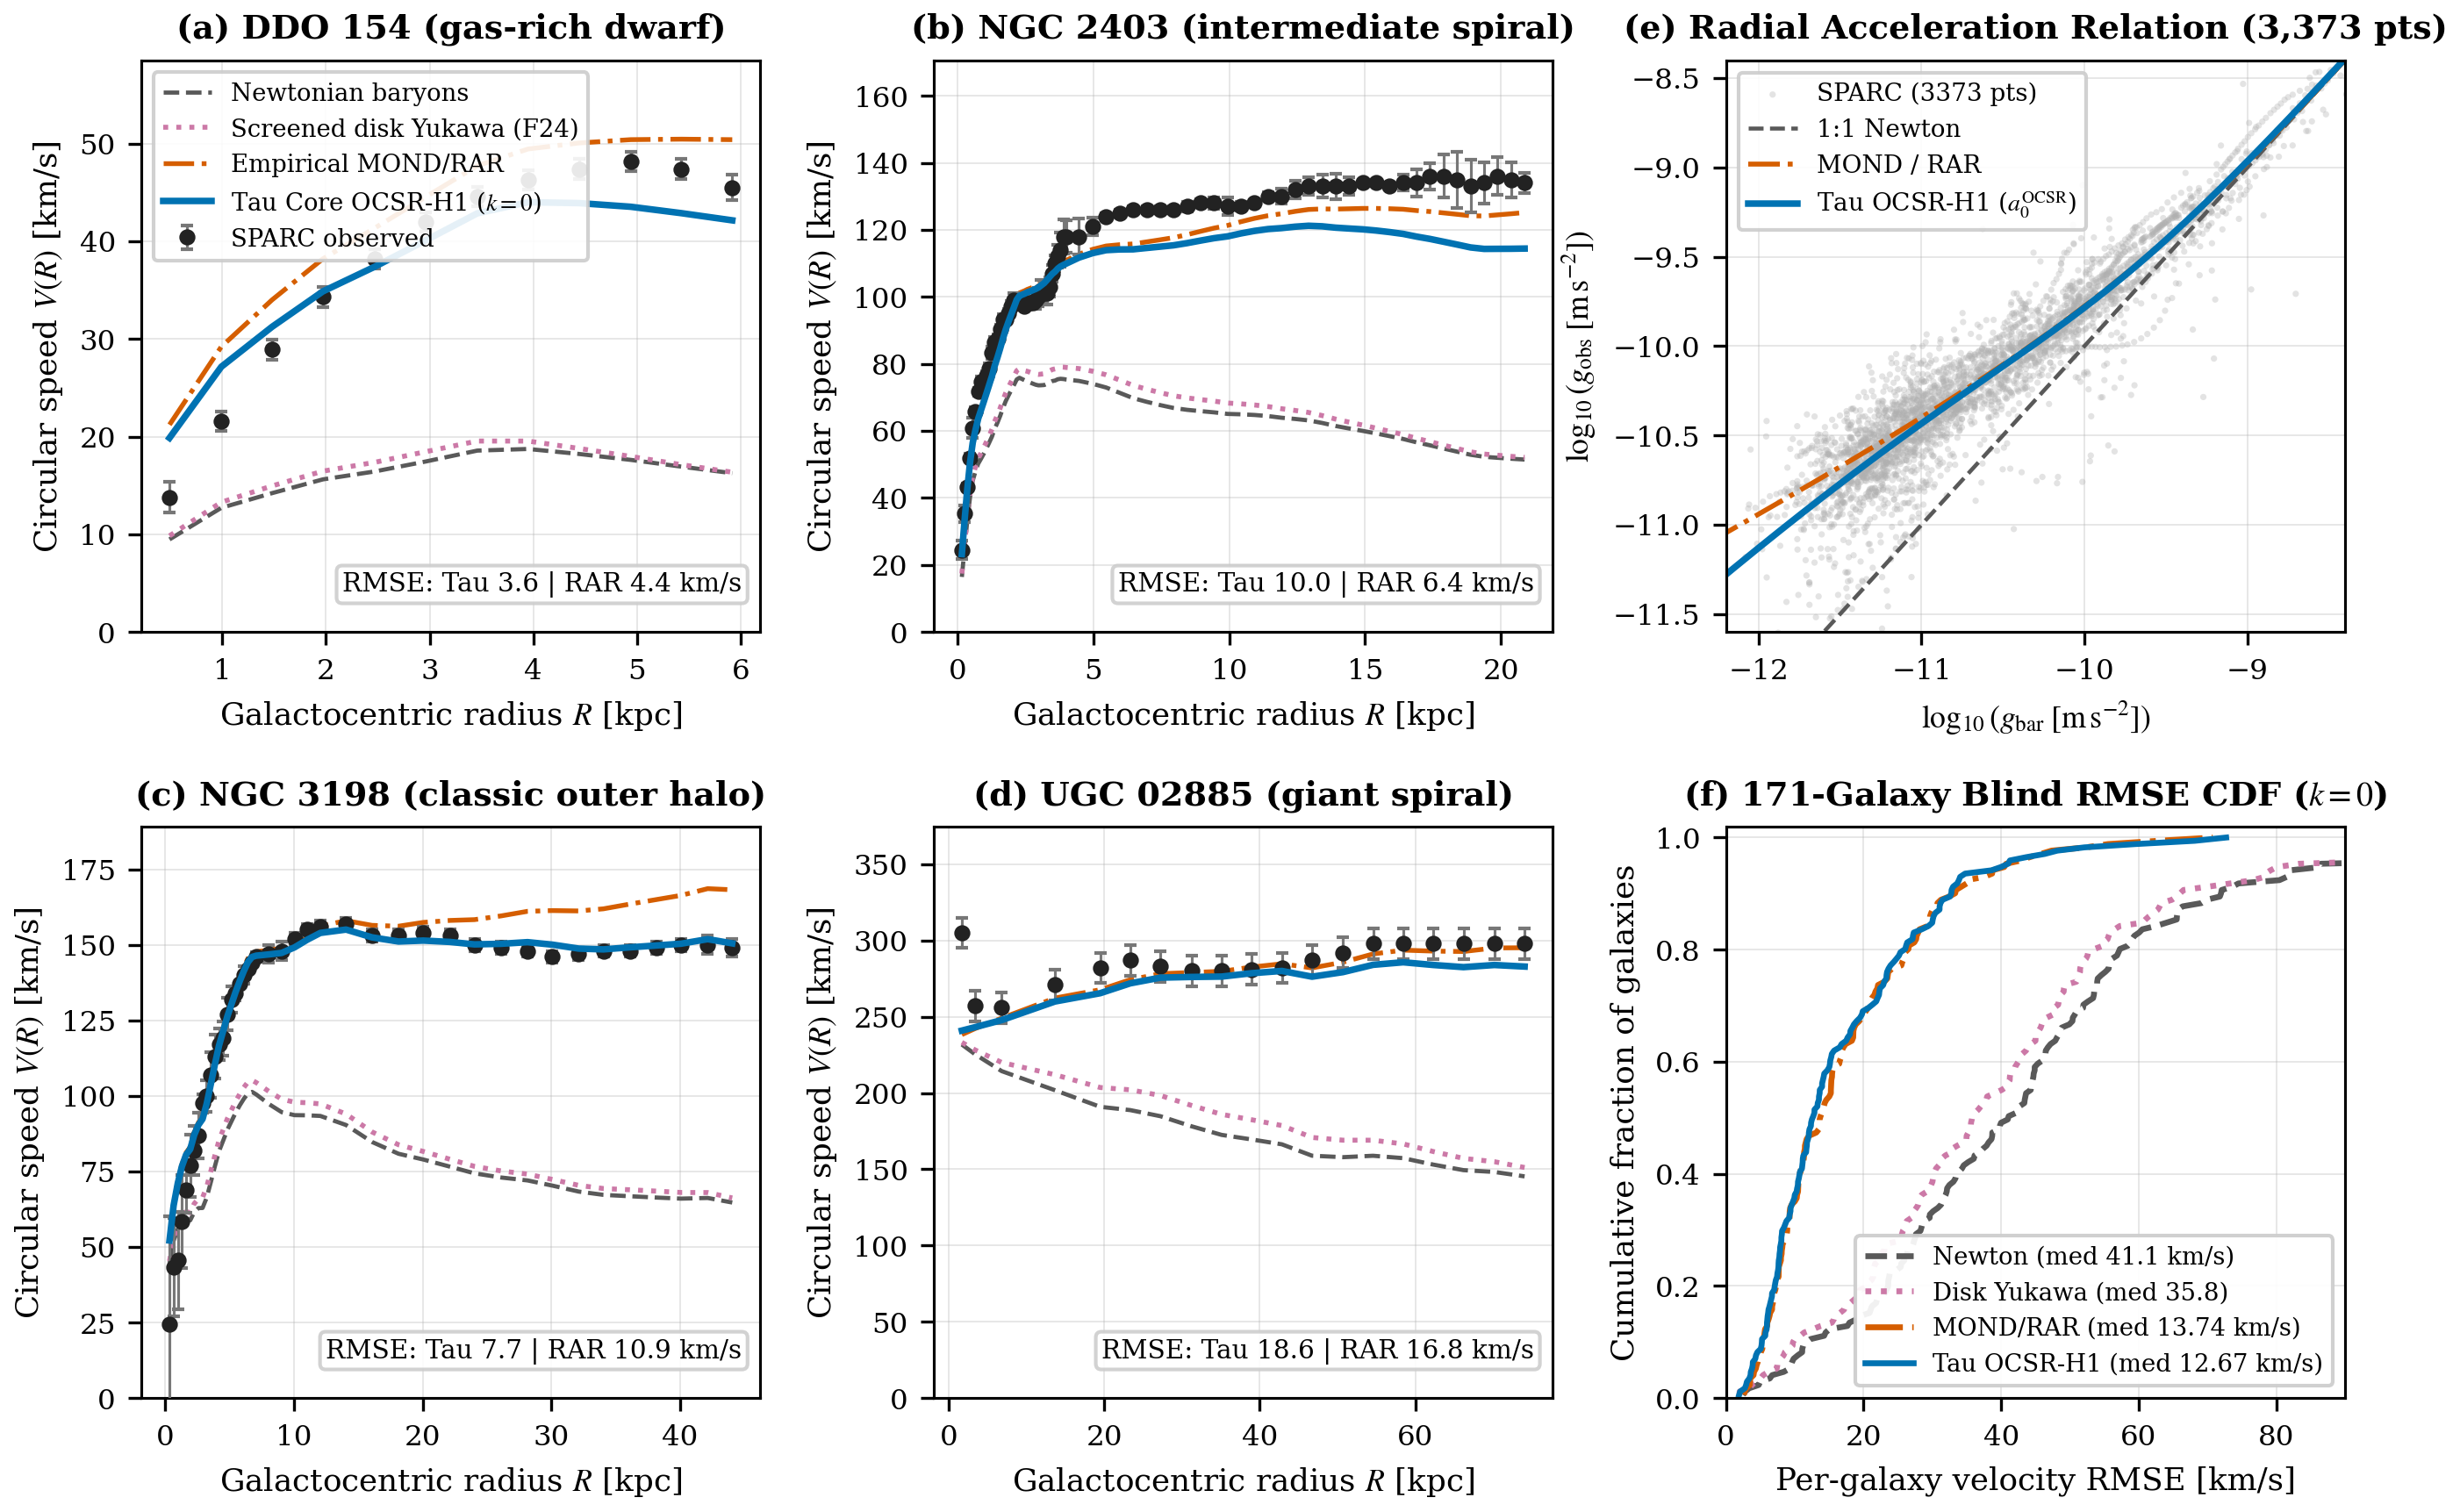
\includegraphics[width=0.98\textwidth]{figures/fig_sparc_rotcurves_and_rar.png}
\caption{Upstream zero-parameter galactic rotation-curve benchmark across the 171-galaxy SPARC sample (\texttt{F24--F28, F37}; shared $\Upsilon_{\mathrm{disk}}=0.5$, $\Upsilon_{\mathrm{bul}}=0.7\,M_\odot/L_\odot$, $k_{\mathrm{gal}}=0$). \textbf{(a--d)} Representative rotation curves (\texttt{DDO 154}, \texttt{NGC 2403}, \texttt{NGC 3198}, \texttt{UGC 02885}) comparing SPARC data $\pm\sigma_V$, Newtonian baryons, screened disk Yukawa (\texttt{F24}), MOND/RAR ($a_{0,\mathrm{emp}}=1.20\times 10^{-10}\;\mathrm{m/s^2}$), and Planck-anchored Tau \texttt{OCSR-H1} ($a_0^{\mathrm{OCSR}}=1.1808\times 10^{-10}\;\mathrm{m/s^2}$). \textbf{(e)} 3,373-point RAR. \textbf{(f)} 171-galaxy RMSE CDF (medians: Tau $12.67\;\mathrm{km/s}$ vs.\ MOND/RAR $13.74\;\mathrm{km/s}$, paired sign-test $p=0.066$, competitive galactic parity without fitting $a_0$).}
\label{fig:paper11-upstream-sparc}
\end{figure}

\begin{figure}[ht!]
\centering
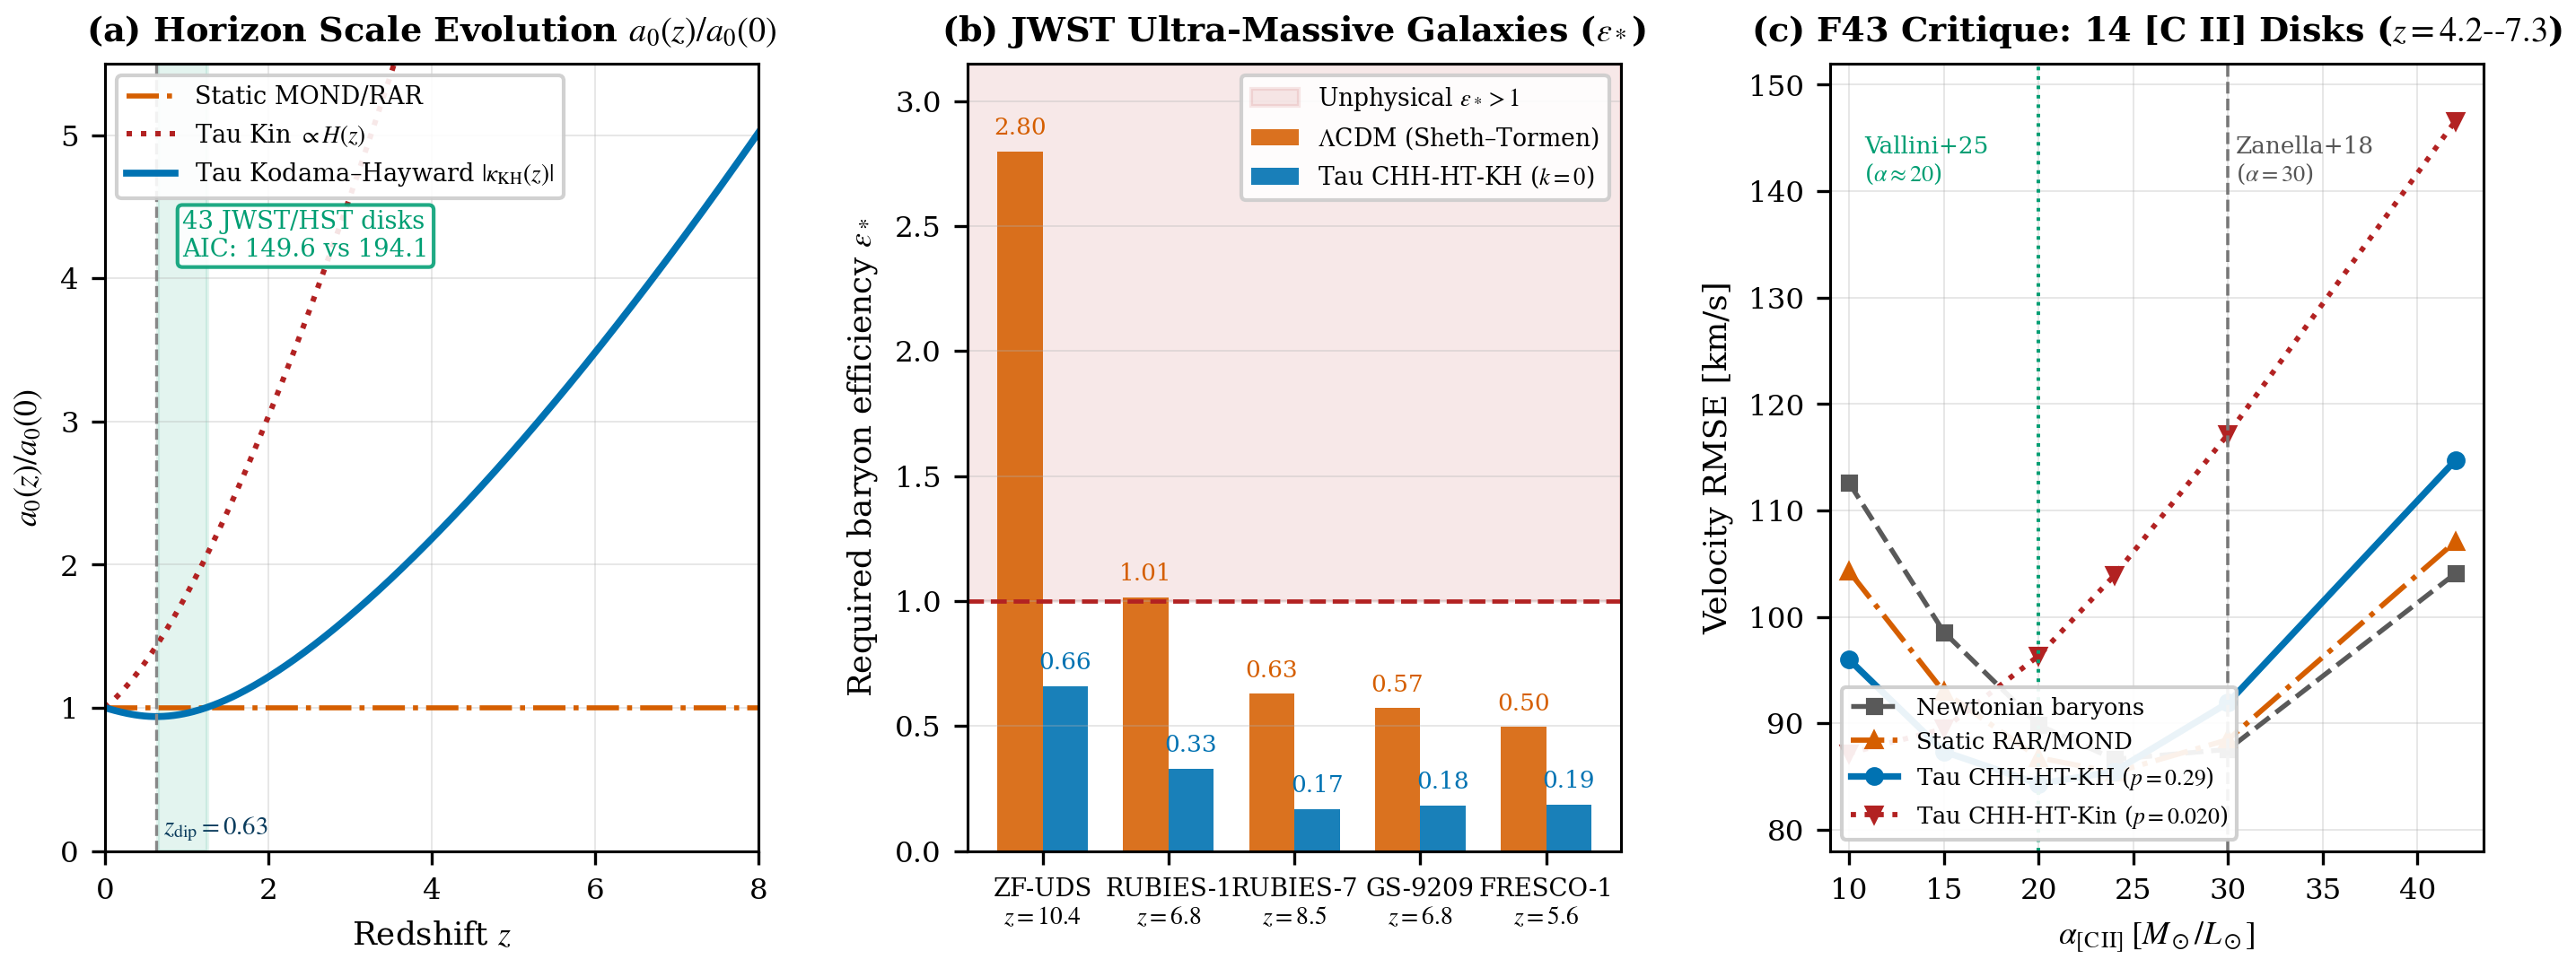
\includegraphics[width=0.98\textwidth]{figures/fig_highz_jwst_a0z_and_cii_audit.png}
\caption{Upstream high-redshift $a_0(z)$ evolution, JWST ultra-massive galaxy baryon efficiency, and self-critical $z>4$ \texttt{[C II]} audit (\texttt{F36, F39, F43}). \textbf{(a)} Normalized Kodama--Hayward $a_0^{\mathrm{KH}}(z)/a_0^{\mathrm{KH}}(0)$ ($z_{\mathrm{dip}}=0.6316$, 43-disk $\mathrm{AIC}=149.6$ vs.\ static RAR $194.1$ and kinematic Tolman $284.8$). \textbf{(b)} Required $\epsilon_*$ on \emph{Nature} 2024 JWST ultra-massive galaxies (\texttt{ZF-UDS-7329}: $2.80\to 0.66$). \textbf{(c)} 14-galaxy $z=4.23\text{--}7.31$ cold \texttt{[C II]} starbursts ($a_N/a_0\simeq 6.9$): Newtonian baryons achieve $87.54\;\mathrm{km/s}$ at $\alpha_{\mathrm{[C\,II]}}=30$, leaving \texttt{Tau KH} ($91.92$) and \texttt{Static RAR} ($88.46$) statistically tied ($p=0.2910$) while rejecting \texttt{Tau Kin} ($117.17$, $p=0.0195$).}
\label{fig:paper11-upstream-highz}
\end{figure}
% END FOUNDATIONS UPDATE 20260929

\section{Conclusion}
\label{sec:conclusion}

We have established a source-frozen, leakage-audited decision protocol for testing whether the declared galaxy-rotation endpoint class requires a dark-sector response layer beyond no-dark Tau morphology/readout ($M_0$), comparing $M_0$ against a Tau base-substrate response family ($M_1$) and a standard dark-sector benchmark ($M_2$). Through canonical revision \texttt{v82}, the protocol verifies SPARC provenance and imports $450$ radial velocity rows across $18$ galaxies, certifies all $72$ prescore four-component leakage checks, emits the non-scored $M_0$ baryonic anchor predictions $v_{\mathrm{body}}(R):=v_{\mathrm{anchor}}(R)$, freezes protocol-local global and per-galaxy privilege counts at zero under the current scaffolds, and enforces level-versus-shape and rank-domain guardrails imported from Paper~10 and the theory hub. Endpoint scoring remains deliberately unactivated pending completion of \path{shared_input_count_discount_policy_v10.csv}, concrete $M_1$ and $M_2$ prediction tables, executable control suites, and pre-registered numerical decision thresholds.

\bibliographystyle{plain}
\bibliography{refs}
\end{document}
